\documentclass[11pt,a4paper]{article}

% --- Page margins, line spacing (20pt), and paragraph spacing ---
\usepackage[margin=1in]{geometry}
\usepackage{setspace}
\setstretch{1.4706} % 13.6pt (11pt default leading) * 1.4706 = 20pt line spacing
\usepackage{parskip}
\usepackage{enumitem}
\setlist{itemsep=3pt, parsep=2pt, topsep=4pt}

% --- Basic math, graphics, and typesetting ---
\usepackage{amsmath,amssymb,amsthm}
\usepackage{xcolor}
\usepackage{tikz}
\usepackage{float}

% --- Custom math operators for clean spacing ---
\DeclareMathOperator{\Arg}{Arg}
\DeclareMathOperator{\Ln}{Ln}
\DeclareMathOperator{\Arcsin}{Arcsin}
\DeclareMathOperator{\Arccos}{Arccos}
\DeclareMathOperator{\Arctan}{Arctan}
\DeclareMathOperator{\Arccot}{Arccot}
\renewcommand{\Re}{\operatorname{Re}}
\renewcommand{\Im}{\operatorname{Im}}

% --- Theorem and definition environments (content starts on a new line) ---
\newtheoremstyle{breakdef}
  {10pt}       % Space above
  {10pt}       % Space below
  {\normalfont}% Body font
  {0pt}        % Indent amount
  {\bfseries}  % Head font
  {.}          % Punctuation after head
  {\newline}   % Line break after head so content starts on the next line
  {}           % Head spec

\newtheoremstyle{breakthm}
  {10pt}       % Space above
  {10pt}       % Space below
  {\itshape}   % Body font
  {0pt}        % Indent amount
  {\bfseries}  % Head font
  {.}          % Punctuation after head
  {\newline}   % Line break after head so content starts on the next line
  {}           % Head spec

\theoremstyle{breakdef}
\newtheorem{definition}{Definition}
\newtheorem{example}{Example}

\theoremstyle{breakthm}
\newtheorem{theorem}{Theorem}
\newtheorem{proposition}{Proposition}
\newtheorem{lemma}{Lemma}
\newtheorem{corollary}{Corollary}

\begin{document}

% ==================================================
% Title and author information
% ==================================================
\begin{center}
    {\LARGE \textbf{Mathematics Method for Physics -- Lecture 04}} \\[0.6em]
    {\large Trigonometric/Inverse Trigonometric Functions, Limits, Continuity, and Differentiability}
\end{center}

\vspace{-0.3em}
\noindent\rule{\textwidth}{0.5pt}
\vspace{0.2em}

\begin{center}
    Instructor: Zhaolong Han, SOCE, Shanghai Jiao Tong University \\
    Email: \texttt{han.arkey@sjtu.edu.cn}
\end{center}

\vspace{0.2em}
\noindent\rule{\textwidth}{0.5pt}

\vspace{0.6em}
\noindent \textit{Lecture notes covering complex trigonometric and inverse trigonometric functions, limits and continuity of complex functions, and differentiability with the Cauchy--Riemann conditions.}

\vspace{1.0em}

% ==================================================
% Section 1: Elementary Complex Functions (Continued)
% ==================================================
\section{Elementary Complex Functions (Continued)}

\subsection{Trigonometric Functions}

\begin{definition}[Complex Sine and Cosine Functions]
Extending Euler's formula $e^{ix} = \cos x + i\sin x$ ($x \in \mathbb{R}$) to any complex number $z \in \mathbb{C}$, the complex sine and cosine functions are defined as
\[
    \sin z = \frac{e^{iz} - e^{-iz}}{2i}, \qquad \cos z = \frac{e^{iz} + e^{-iz}}{2}.
\]
The remaining trigonometric functions are defined analogously:
\[
    \tan z = \frac{\sin z}{\cos z}, \quad \cot z = \frac{\cos z}{\sin z}, \quad \sec z = \frac{1}{\cos z}, \quad \csc z = \frac{1}{\sin z}.
\]
\end{definition}

\textbf{Key Properties:}
\begin{enumerate}
    \item \textbf{Periodicity and Parity}: Both $\sin z$ and $\cos z$ are periodic with fundamental period $2\pi$:
    \[
        \sin(z + 2\pi) = \sin z, \qquad \cos(z + 2\pi) = \cos z.
    \]
    Moreover, $\sin(-z) = -\sin z$ (odd) and $\cos(-z) = \cos z$ (even).
    \item \textbf{Trigonometric Identities}: Standard identities from real analysis remain valid for all $z, z_1, z_2 \in \mathbb{C}$, including Euler's formula $e^{iz} = \cos z + i\sin z$, the Pythagorean identity
    \[
        \sin^2 z + \cos^2 z = 1,
    \]
    and the sum/difference formulas $\sin(z_1 \pm z_2) = \sin z_1 \cos z_2 \pm \cos z_1 \sin z_2$ and $\cos(z_1 \pm z_2) = \cos z_1 \cos z_2 \mp \sin z_1 \sin z_2$.
    \item \textbf{Zeros}: $\sin z = 0 \iff z = k\pi$, and $\cos z = 0 \iff z = k\pi + \frac{\pi}{2}$ ($k \in \mathbb{Z}$). All zeros lie on the real axis.
    \item \textbf{Failure of Boundedness}: Unlike real sine and cosine, the inequalities $|\sin z| \le 1$ and $|\cos z| \le 1$ \textbf{no longer hold} in the complex plane. In fact, $|\sin z|$ and $|\cos z|$ are unbounded on $\mathbb{C}$ (for instance, $|\cos(iy)| = \cosh y \to +\infty$ as $|y| \to \infty$).
\end{enumerate}

\begin{example}[Solving a Complex Trigonometric Equation]
Solve the equation $\sin z = 2$ in $\mathbb{C}$.

\textbf{Solution:} Using the exponential definition of $\sin z$, we write
\[
    \sin z = \frac{e^{iz} - e^{-iz}}{2i} = 2 \implies e^{iz} - e^{-iz} - 4i = 0.
\]
Multiplying through by $e^{iz}$ yields a quadratic equation in $X = e^{iz}$:
\[
    (e^{iz})^2 - 4i(e^{iz}) - 1 = 0.
\]
Applying the quadratic formula ($aX^2 + bX + c = 0$ with $a = 1$, $b = -4i$, and $c = -1$):
\[
    e^{iz} = \frac{-(-4i) \pm \sqrt{(-4i)^2 - 4(1)(-1)}}{2(1)} = \frac{4i \pm \sqrt{-16 + 4}}{2} = \frac{4i \pm 2\sqrt{3}i}{2} = (2 \pm \sqrt{3})i.
\]
Taking the complex logarithm on both sides gives
\begin{align*}
    iz &= \Ln\bigl[(2 \pm \sqrt{3})i\bigr] = \ln\bigl|(2 \pm \sqrt{3})i\bigr| + i\Arg\bigl[(2 \pm \sqrt{3})i\bigr] \\
       &= \ln(2 \pm \sqrt{3}) + i\left(\frac{\pi}{2} + 2k\pi\right) \quad (k = 0, \pm 1, \pm 2, \dots).
\end{align*}
Multiplying both sides by $-i$ and noting that $\ln(2 - \sqrt{3}) = -\ln(2 + \sqrt{3})$, we obtain
\[
    z = \frac{\pi}{2} + 2k\pi - i\ln(2 \pm \sqrt{3}) = \frac{\pi}{2} + 2k\pi \mp i\ln(2 + \sqrt{3}) \quad (k = 0, \pm 1, \pm 2, \dots).
\]
\end{example}

\subsection{Inverse Trigonometric Functions}

\begin{definition}[Inverse Trigonometric Functions]
Defined as the inverse relations of the complex trigonometric functions (such as $w = \Arcsin z \iff \sin w = z$), the inverse trigonometric functions are infinitely many-valued and are expressed in terms of the complex logarithm as follows:
\begin{align*}
    w &= \Arcsin z = -i\Ln\left(iz \pm \sqrt{1 - z^2}\right), \\
    w &= \Arccos z = -i\Ln\left(z \pm \sqrt{z^2 - 1}\right), \\
    w &= \Arctan z = -\frac{i}{2}\Ln\frac{1 + iz}{1 - iz} \quad (z \neq \pm i), \\
    w &= \Arccot z = \frac{i}{2}\Ln\frac{z - i}{z + i} \quad (z \neq \pm i).
\end{align*}
\end{definition}

\textit{Derivation sketch for $\Arcsin z$}: From $z = \sin w = \frac{e^{iw} - e^{-iw}}{2i}$, we obtain $e^{2iw} - 2ize^{iw} - 1 = 0$. Solving this quadratic equation for $e^{iw}$ yields $e^{iw} = iz \pm \sqrt{1 - z^2}$, and taking $\Ln$ gives $w = -i\Ln(iz \pm \sqrt{1 - z^2})$.

% ==================================================
% Section 2: Limits and Continuity of Complex Functions
% ==================================================
\section{Limits and Continuity of Complex Functions}

\subsection{Limit of a Complex Function}

\begin{definition}[Limit at a Point]
Let $w = f(z)$ be defined in a deleted neighborhood of $z_0$, and let $A \in \mathbb{C}$ be a complex constant. If for every $\varepsilon > 0$, there exists a $\delta > 0$ such that
\[
    0 < |z - z_0| < \delta \implies |f(z) - A| < \varepsilon,
\]
then $A$ is called the \textbf{limit} of $f(z)$ as $z$ approaches $z_0$, denoted by
\[
    \lim_{z \to z_0} f(z) = A \quad (\text{or } f(z) \to A \text{ as } z \to z_0).
\]
\end{definition}

\textbf{Geometric Remark}: In one-dimensional real calculus, $x \to x_0$ can only occur from two directions ($x \to x_0^+$ or $x \to x_0^-$). In the complex plane, however, $z \to z_0$ corresponds to $(x, y) \to (x_0, y_0)$ in $\mathbb{R}^2$, which can happen along \textbf{infinitely many arbitrary paths and directions}. For $\lim_{z \to z_0} f(z) = A$ to exist, $f(z)$ must approach $A$ regardless of the path taken by $z \to z_0$.

\begin{theorem}[Reduction to Real Two-Variable Limits]
Let $z = x + iy$, $z_0 = x_0 + iy_0$, $w = f(z) = u(x, y) + iv(x, y)$, and $A = a + bi$. Then
\[
    \lim_{z \to z_0} f(z) = A \iff \lim_{(x,y) \to (x_0,y_0)} u(x, y) = a \quad \text{and} \quad \lim_{(x,y) \to (x_0,y_0)} v(x, y) = b.
\]
\end{theorem}

\textbf{Algebraic Properties of Limits}: If $\lim_{z \to z_0} f(z) = A$ and $\lim_{z \to z_0} g(z) = B$, then:
\[
    \lim_{z \to z_0} [f(z) \pm g(z)] = A \pm B, \quad \lim_{z \to z_0} [f(z)g(z)] = AB, \quad \lim_{z \to z_0} \frac{f(z)}{g(z)} = \frac{A}{B} \quad (B \neq 0).
\]

\subsection{Continuity of a Complex Function}

\begin{definition}[Continuity]
Let $w = f(z)$ be a complex function defined in a neighborhood of $z_0$ or a domain $D$:
\begin{enumerate}
    \item \textbf{Continuity at a Point}: $f(z)$ is said to be \textbf{continuous at $z_0$} if
    \[
        \lim_{z \to z_0} f(z) = f(z_0).
    \]
    \item \textbf{Continuity in a Domain}: $f(z)$ is said to be \textbf{continuous in a domain $D$} if it is continuous at every point $z_0 \in D$.
\end{enumerate}
\end{definition}

\begin{theorem}[Continuity via Real and Imaginary Parts]
A function $f(z) = u(x, y) + iv(x, y)$ is continuous at $z_0 = x_0 + iy_0$ if and only if both real functions $u(x, y)$ and $v(x, y)$ are continuous at $(x_0, y_0)$.
\end{theorem}

Sums, differences, products, quotients (with non-zero denominators), and compositions of continuous complex functions remain continuous. Furthermore, if $f(z)$ is continuous on a bounded closed domain $\overline{D}$, then $|f(z)|$ is bounded on $\overline{D}$ and attains its maximum and minimum values.

\begin{example}[Continuity Analysis of $w = \arg z$]
Discuss the continuity of the principal argument function $w = \arg z \in (-\pi, \pi]$ on the complex plane.

\textbf{Solution:} For $z = x + iy \neq 0$, $\arg z$ is given explicitly by
\[
    \arg z = \begin{cases}
        \arctan\dfrac{y}{x}, & x > 0, \\[0.9em]
        \pi + \arctan\dfrac{y}{x}, & x < 0, \, y \ge 0, \\[0.9em]
        -\pi + \arctan\dfrac{y}{x}, & x < 0, \, y < 0, \\[0.9em]
        \pm\dfrac{\pi}{2}, & x = 0, \, y \gtrless 0.
    \end{cases}
\]
\begin{itemize}
    \item At $z = 0$, $\arg z$ is undefined, so it is discontinuous at the origin.
    \item Let $z_0 = x_0 < 0$ be any point on the negative real axis. Approaching $x_0$ from the upper half-plane ($\Im z > 0$) versus the lower half-plane ($\Im z < 0$) yields different directional limits:
    \[
        \lim_{\substack{z \to x_0 \\ \Im z > 0}} \arg z = \pi, \qquad \lim_{\substack{z \to x_0 \\ \Im z < 0}} \arg z = -\pi.
    \]
    \item Since these limits do not agree, $\lim_{z \to x_0} \arg z$ does not exist, proving that $\arg z$ is discontinuous at every point on the negative real axis.
\end{itemize}
\textbf{Conclusion}: $w = \arg z$ is continuous everywhere on the \textbf{slit complex plane} $\mathbb{C} \setminus (-\infty, 0]$ (the complex plane cut along the non-positive real axis).
\end{example}

\begin{figure}[H]
\centering
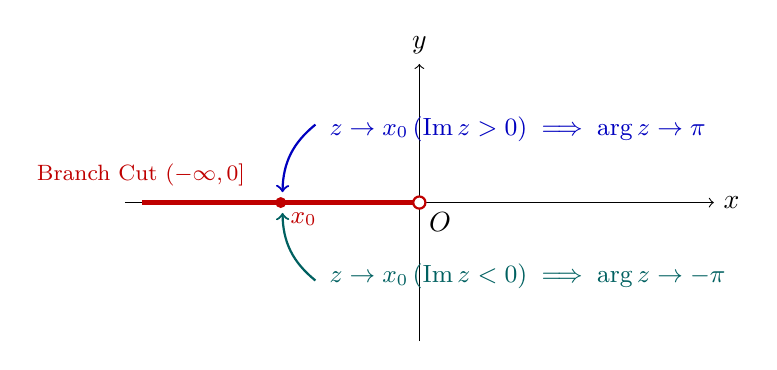
\begin{tikzpicture}[scale=1.1]
    % Axes
    \draw[->] (-3.4, 0) -- (3.4, 0) node[right] {$x$};
    \draw[->] (0, -1.6) -- (0, 1.6) node[above] {$y$};

    % Branch cut along negative real axis (-infty, 0]
    \draw[ultra thick, red!75!black] (-3.2, 0) -- (0, 0);
    \fill[white] (0,0) circle (2pt);
    \draw[thick, red!75!black] (0,0) circle (2pt);
    \node[below right] at (0,0) {$O$};

    % Point x0 < 0 on negative real axis
    \coordinate (x0) at (-1.6, 0);
    \fill[red!75!black] (x0) circle (1.8pt) node[below right, font=\small] {$x_0$};

    % Upper approach
    \draw[->, thick, blue!75!black] (-1.2, 0.9) to[bend right=25] (-1.58, 0.12);
    \node[blue!75!black, right, font=\small] at (-1.15, 0.85) {$z \to x_0 \, (\Im z > 0) \implies \arg z \to \pi$};

    % Lower approach
    \draw[->, thick, teal!75!black] (-1.2, -0.9) to[bend left=25] (-1.58, -0.12);
    \node[teal!75!black, right, font=\small] at (-1.15, -0.85) {$z \to x_0 \, (\Im z < 0) \implies \arg z \to -\pi$};

    \node[red!75!black, above left, font=\footnotesize] at (-1.9, 0.08) {Branch Cut $(-\infty, 0]$};
\end{tikzpicture}
\caption{Jump discontinuity of $\arg z$ across the branch cut $(-\infty, 0]$.}
\end{figure}

% ==================================================
% Section 3: Differentiability and Cauchy-Riemann Conditions
% ==================================================
\section{Differentiability and Cauchy--Riemann Conditions}

\subsection{Derivative and Differential of a Complex Function}

\begin{definition}[Derivative of a Complex Function]
Let $w = f(z)$ be defined in a neighborhood of $z_0$. If the limit
\[
    \lim_{\Delta z \to 0} \frac{f(z_0 + \Delta z) - f(z_0)}{\Delta z} = \lim_{z \to z_0} \frac{f(z) - f(z_0)}{z - z_0}
\]
exists, then $f(z)$ is said to be \textbf{differentiable at $z_0$}, and this limit is called the \textbf{derivative} of $f(z)$ at $z_0$, denoted by $f'(z_0)$ or $\left.\frac{dw}{dz}\right|_{z=z_0}$.
\end{definition}

\begin{definition}[Differential of a Complex Function]
A function $f(z)$ is differentiable at $z_0$ if and only if its increment $\Delta f(z_0) = f(z_0 + \Delta z) - f(z_0)$ can be expressed as
\[
    \Delta f(z_0) = A \Delta z + o(\Delta z), \qquad \text{where } \lim_{\Delta z \to 0} \frac{o(\Delta z)}{\Delta z} = 0.
\]
Here $A = f'(z_0)$, and the principal linear part $df = A \Delta z = f'(z_0)\Delta z = f'(z_0)dz$ is called the \textbf{differential} of $f(z)$ at $z_0$.
\end{definition}

\textbf{Remarks}:
\begin{itemize}
    \item Because $\Delta z \to 0$ must yield the same limit along \emph{all} paths in $\mathbb{C}$, complex differentiability is far more restrictive than real differentiability.
    \item If $f(z)$ is differentiable at $z_0$, it is necessarily continuous at $z_0$; the converse is false (e.g., $f(z) = \overline{z}$ and $f(z) = \Im z$ are continuous everywhere but differentiable nowhere; $f(z) = |z|^2$ is differentiable only at $z = 0$).
    \item Standard differentiation rules (linearity, product rule, quotient rule, chain rule, and inverse function rule) hold identically to real calculus.
\end{itemize}

\subsection{Necessary Condition: The Cauchy--Riemann Equations}

\begin{theorem}[Necessary Condition for Differentiability]
Suppose $f(z) = u(x, y) + iv(x, y)$ is differentiable at $z_0 = x_0 + iy_0$. Then the first-order partial derivatives $u_x, u_y, v_x, v_y$ exist at $(x_0, y_0)$ and satisfy the \textbf{Cauchy--Riemann (C--R) equations}:
\[
    \begin{cases}
        u_x = v_y, \\
        u_y = -v_x,
    \end{cases}
    \qquad \text{i.e.,} \qquad
    \frac{\partial u}{\partial x} = \frac{\partial v}{\partial y}, \quad \frac{\partial u}{\partial y} = -\frac{\partial v}{\partial x}.
\]
Furthermore, the derivative at $z_0$ is given by
\[
    f'(z_0) = \frac{\partial u}{\partial x} + i\frac{\partial v}{\partial x} = \frac{\partial v}{\partial y} - i\frac{\partial u}{\partial y}.
\]
\end{theorem}

\begin{proof}
Let $\Delta z = z - z_0 = \Delta x + i\Delta y$ and $\Delta w = f(z) - f(z_0) = \Delta u + i\Delta v$, where
\[
    \Delta u = u(x_0 + \Delta x, y_0 + \Delta y) - u(x_0, y_0), \qquad \Delta v = v(x_0 + \Delta x, y_0 + \Delta y) - v(x_0, y_0).
\]
Since $f'(z_0)$ exists, the limit
\[
    f'(z_0) = \lim_{\Delta z \to 0} \frac{\Delta u + i\Delta v}{\Delta x + i\Delta y}
\]
is independent of how $\Delta z \to 0$:
\begin{enumerate}
    \item \textbf{Horizontal path} ($\Delta y = 0$, $\Delta x \to 0$):
    \[
        f'(z_0) = \lim_{\Delta x \to 0} \frac{\Delta u + i\Delta v}{\Delta x + i\cdot 0} = \lim_{\Delta x \to 0} \left(\frac{\Delta u}{\Delta x} + i\frac{\Delta v}{\Delta x}\right) = \frac{\partial u}{\partial x} + i\frac{\partial v}{\partial x}.
    \]
    \item \textbf{Vertical path} ($\Delta x = 0$, $\Delta y \to 0$):
    \[
        f'(z_0) = \lim_{\Delta y \to 0} \frac{\Delta u + i\Delta v}{0 + i\Delta y} = \lim_{\Delta y \to 0} \left(\frac{\Delta v}{\Delta y} - i\frac{\Delta u}{\Delta y}\right) = \frac{\partial v}{\partial y} - i\frac{\partial u}{\partial y}.
    \]
\end{enumerate}
Equating the real and imaginary parts of these two expressions yields $u_x = v_y$ and $u_y = -v_x$ at $(x_0, y_0)$.
\end{proof}

\begin{figure}[H]
\centering
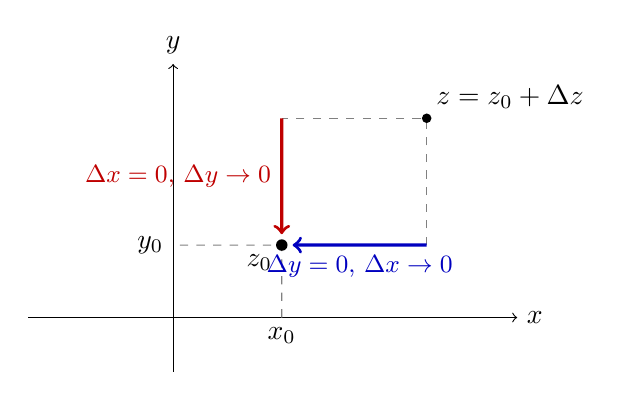
\begin{tikzpicture}[scale=1.15]
    \draw[->] (-1.6, 0) -- (3.8, 0) node[right] {$x$};
    \draw[->] (0, -0.6) -- (0, 2.8) node[above] {$y$};

    \coordinate (z0) at (1.2, 0.8);
    \coordinate (z1) at (2.8, 0.8);
    \coordinate (z2) at (1.2, 2.2);
    \coordinate (z)  at (2.8, 2.2);

    \draw[dashed, gray] (1.2, 0) node[below, black] {$x_0$} -- (z0) -- (0, 0.8) node[left, black] {$y_0$};
    \draw[dashed, gray] (z1) -- (z) -- (z2);

    % Horizontal path
    \draw[->, very thick, blue!75!black] (z1) -- (1.32, 0.8) node[midway, below, font=\small] {$\Delta y = 0, \, \Delta x \to 0$};
    % Vertical path
    \draw[->, very thick, red!75!black] (z2) -- (1.2, 0.92) node[midway, left, font=\small] {$\Delta x = 0, \, \Delta y \to 0$};

    \fill[black] (z0) circle (1.8pt) node[below left] {$z_0$};
    \fill[black] (z) circle (1.5pt) node[above right] {$z = z_0 + \Delta z$};
\end{tikzpicture}
\caption{Horizontal and vertical approach paths used to derive the Cauchy--Riemann equations.}
\end{figure}

\textit{Remark (Polar Form)}: In polar coordinates $z = re^{i\theta}$, the Cauchy--Riemann equations take the form
\[
    \frac{\partial u}{\partial r} = \frac{1}{r}\frac{\partial v}{\partial \theta}, \qquad \frac{\partial v}{\partial r} = -\frac{1}{r}\frac{\partial u}{\partial \theta}, \qquad f'(z) = e^{-i\theta}\left(\frac{\partial u}{\partial r} + i\frac{\partial v}{\partial r}\right).
\]

\subsection{Counterexample: C--R Equations Alone Are Not Sufficient}

\begin{example}[Non-differentiable Function Satisfying C--R Equations]
Examine the differentiability of $f(z) = \sqrt{|xy|}$ at the origin $z_0 = 0$.

\textbf{Solution:} Here $u(x, y) = \sqrt{|xy|}$ and $v(x, y) = 0$. Computing the first-order partial derivatives at $(0, 0)$ by definition:
\begin{align*}
    u_x(0, 0) &= \lim_{\Delta x \to 0} \frac{u(\Delta x, 0) - u(0, 0)}{\Delta x} = \lim_{\Delta x \to 0} \frac{0 - 0}{\Delta x} = 0, \\
    u_y(0, 0) &= \lim_{\Delta y \to 0} \frac{u(0, \Delta y) - u(0, 0)}{\Delta y} = \lim_{\Delta y \to 0} \frac{0 - 0}{\Delta y} = 0, \\
    v_x(0, 0) &= 0, \qquad v_y(0, 0) = 0.
\end{align*}
Thus, $u_x = v_y = 0$ and $u_y = -v_x = 0$ at $(0, 0)$, so the Cauchy--Riemann equations are satisfied. However, evaluating the difference quotient along the straight line $y = kx$ as $x \to 0$ gives
\[
    \lim_{\Delta z \to 0} \frac{f(z) - f(0)}{z - 0} = \lim_{x \to 0} \frac{\sqrt{|kx^2|}}{x + ikx} = \lim_{x \to 0} \frac{|x|\sqrt{|k|}}{x(1 + ik)},
\]
which depends on the slope $k$ (and the sign of $x$). Therefore, $\lim_{\Delta z \to 0} \frac{\Delta f}{\Delta z}$ does not exist, and $f(z) = \sqrt{|xy|}$ is \textbf{not differentiable} at $z = 0$.
\end{example}

\subsection{Necessary and Sufficient Condition for Differentiability}

\begin{theorem}[Necessary and Sufficient Condition for Differentiability]
A complex function $w = f(z) = u(x, y) + iv(x, y)$ defined in a domain $D$ is differentiable at $z = x + iy \in D$ if and only if:
\begin{enumerate}
    \item $u(x, y)$ and $v(x, y)$ are \textbf{differentiable} (as real functions of two variables) at $(x, y)$; and
    \item $u(x, y)$ and $v(x, y)$ satisfy the \textbf{Cauchy--Riemann equations} ($u_x = v_y$, $u_y = -v_x$) at $(x, y)$.
\end{enumerate}
\end{theorem}

\begin{proof}
Let $\Delta z = \Delta x + i\Delta y$, $\Delta w = \Delta u + i\Delta v$, $A = \alpha + i\beta$, and $o(\Delta z) = \varepsilon_1 + i\varepsilon_2$ (where $\varepsilon_1, \varepsilon_2 = o(|\Delta z|)$). By definition, $w = f(z)$ is differentiable at $z$ if and only if
\[
    \Delta w = A\Delta z + o(\Delta z) \iff \Delta u + i\Delta v = (\alpha + i\beta)(\Delta x + i\Delta y) + \varepsilon_1 + i\varepsilon_2,
\]
which is equivalent to the real system
\[
    \begin{cases}
        \Delta u = \alpha \Delta x - \beta \Delta y + \varepsilon_1, \\
        \Delta v = \beta \Delta x + \alpha \Delta y + \varepsilon_2,
    \end{cases}
    \qquad \text{with } \varepsilon_1, \varepsilon_2 = o\left(\sqrt{\Delta x^2 + \Delta y^2}\right).
\]
This holds if and only if $u(x, y)$ and $v(x, y)$ are real-differentiable at $(x, y)$ with partial derivatives $\alpha = u_x = v_y$ and $-\beta = u_y = -v_x$, i.e., $u$ and $v$ satisfy the Cauchy--Riemann equations at $(x, y)$, in which case $f'(z) = \alpha + i\beta = u_x + iv_x$.
\end{proof}

\begin{corollary}[Sufficient Condition for Differentiability]
If $u(x, y)$ and $v(x, y)$ have \textbf{continuous} first-order partial derivatives at $(x, y)$ and satisfy the Cauchy--Riemann equations there, then $f(z) = u(x, y) + iv(x, y)$ is differentiable at $z = x + iy$.
\end{corollary}

% ==================================================
% Assigned Exercises Reference
% ==================================================
\section*{Assigned Homework Reference}
\begin{itemize}
    \item \textbf{Textbook P.53 (Exercise 2)}: Set A: Problems 1 (even), 2, 3, 4, 13 (even), 15.
\end{itemize}

\end{document}